\chapter{Euristici}\label{sec:capheur}
Analizziamo infine alcune tecniche euristiche usate per calcolare una soluzione ammissibile, anche se in generale subottima, da impiegare come punto di partenza per il subgradiente lagrangiano, il branch-and-bound o una risoluzione basata su MIP, ma anche per calcolare una soluzione a sé stante. In questa sezione esponiamo e confrontiamo euristici basati sia sulla formulazione generale del problema, sia sul modello MIP.

\section{Euristici basati sulla formulazione del problema}
\subsection{Nearest Neighbour}
Il primo euristico che analizziamo è anche quello forse più intuitivo, l’algoritmo Nearest Neighbour (NN). Partendo da un nodo qualsiasi, l’algoritmo esegue una scelta greedy scegliendo l’arco di costo minimo tra quelli che collegano il nodo a nodi non già precedentemente visitati, fino a che tutti i nodi non sono stati visitati, al che l’algoritmo ritorna al nodo di partenza con l’unico arco possibile.

L’idea è molto semplice e ``naturale’’, ma la scelta localmente ottima può, nel corso delle iterazioni, spingere l’algoritmo verso zone in cui ci sono diversi nodi molto vicini, costringendo poi la selezione di archi di costo elevato per muoversi verso i rimanenti nodi del grafo. Ciò risulta evidente osservando il risultato dell’esecuzione dell’algoritmo su un grafo, quando si notano archi che attraversano lunghi tratti per collegare due nodi distanti tra loro. Una possibile idea per attenuare in parte il problema è quella di eseguire più volte la ricerca, partendo da diversi nodi del grafo.

\subsection{$k$-opt}
\begin{figure}
  \begin{center}
    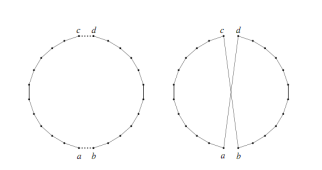
\includegraphics[width=0.6\textwidth]{images/2opt}
    \caption{Scambio di archi in 2-opt.}
    \label{fig:2opt}
  \end{center}
\end{figure}
Un’idea molto naturale che nasce dall’osservazione del risultato dell’algoritmo NN su istanze del TSP, o perlomeno su istanze del TSP che rispettano la disuguaglianza triangolare, è quella di scambiare due archi che si incrociano, secondo l’operazione in figura \ref{fig:2opt}. Tale operazione è chiamata 2-opt (\citet*{croes1958method}). Il risultato è quello di collegare in maniera localmente ottima due coppie di nodi.

Questa procedura può essere estesa a più coppie di nodi. Ad esempio, lo scambio di archi tra 3 coppie di nodi è detta 3-opt, e, in generale, su $k$ coppie di nodi si definisce un’operazione $k$-opt. Queste operazioni sono applicabili a qualsiasi tour hamiltoniano, per migliorare la soluzione corrente, ottenuta con un algoritmo euristico. Nel nostro caso abbiamo applicato 2-opt e 3-opt a cicli ottenuti con NN, e a cicli generati in maniera casuale. Nel primo caso l’idea è quella di migliorare una soluzione che si suppone già sufficientemente buona. Nel secondo caso invece di ottiene un circuito in genere pessimo dal punto di vista del costo, e molto intricato se osservato, ma molto veloce da calcolare e che può essere migliorato di molto; questo permette di generare moltissimi cicli e testare il loro ``potenziale’’ applicando gli step di $k$-ottimalità in un tempo relativamente contenuto. Quest'ultimo procedimento è chiamato di seguito RC, per random cycle.

Le figure \ref{fig:nn}--\ref{fig:nn23opt} mostrano le differenze tra NN, NN+2-opt, e NN+23opt.

\begin{figure}
  \begin{center}
    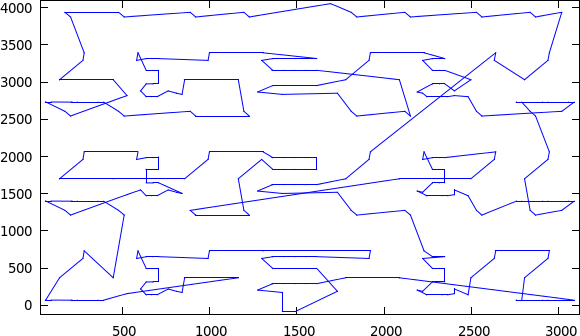
\includegraphics[width=0.7\textwidth]{images/lin318nn}
    \caption{Risultato di NN per \texttt{lin318}.}
    \label{fig:nn}

    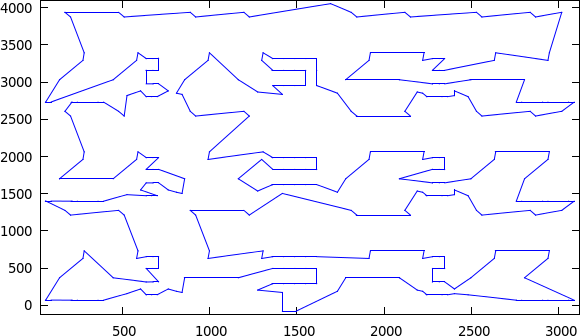
\includegraphics[width=0.7\textwidth]{images/lin318nn2opt}
    \caption{Risultato di NN+2opt per \texttt{lin318}.}
    \label{fig:nn2opt}
  
    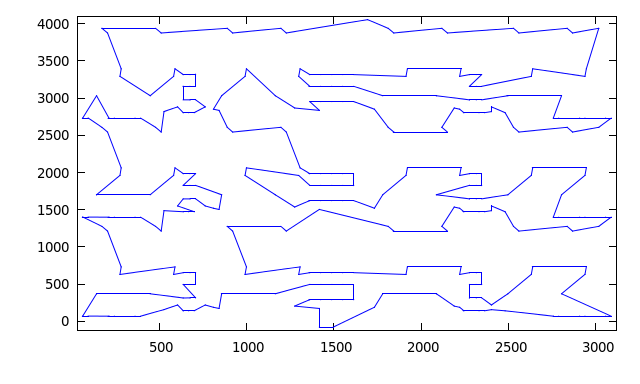
\includegraphics[width=0.7\textwidth]{images/lin318nn23opt}
    \caption{Risultato di NN+23opt per \texttt{lin318}.}
    \label{fig:nn23opt}
  \end{center}
\end{figure}

Dal punto di vista teorico le operazioni $k$-opt costituiscono una ricerca locale in un intorno della soluzione corrente. Non sono quindi garantiti il raggiungimento della soluzione ottima, né la sua certificazione come tale. Al crescere di k la ricerca si estende a intorni di raggio sempre maggiore, a scapito tuttavia del tempo di calcolo e della complessità dell’algoritmo, che già per $k=3$ diventa molto oneroso. Queste procedure sono comunque alla base degli euristici Lin-Kernighan (\citet*{lin1973effective}) e Lin-Kernighan-Helsgaun (\citet*{helsgaun2000effective}), ad oggi i più efficaci euristici per il TSP in letteratura.

\subsection{Branch-and-bound con prefissaggio}
Abbiamo inoltre provato un approccio ispirato a RINS (si veda la sezione \ref{sec:rins}), basato sulle soluzioni calcolate dall’euristico di partenza. L’idea è valutare le soluzioni calcolate ad ogni iterazione dell’euristico (in particolare RC+2opt, che genera molti cicli potenzialmente diversi, mentre NN+2opt restituirà un numero limitato di cicli distinti) e confidare nel fatto che gli archi selezionati in tutte le iterazioni sono parte della soluzione ottima; allo stesso modo, gli archi sempre scartati da tutte le iterazioni dell’euristico sono considerati esclusi anche dalla soluzione ottima. Vengono così fissate a zero le variabili corrispondenti agli archi scartati, e a 1 le variabili relative agli archi sempre presenti nelle varie soluzioni. Viene quindi lanciato il branch-and-bound, che agirà sulle variabili non fissate.

Ovviemente, non c’è nessuna garanzia che questo metodo porti alla soluzione ottima (basti pensare al caso limite in cui viene eseguita una sola iterazione dell’euristico: tutte le variabili verranno fissate al valore che assumono nella soluzione euristica, il branch-and-bound non ha gradi di libertà, e la soluzione ritornata sarà quella calcolata dall’euristico), ma possiamo sperare che se molte iterazioni concordano su alcune variabili, il loro valore sarà molto probabilmente lo stesso della soluzione ottima.

\section{Euristici basati su modello MIP}
L’altra tipologia di euristici che abbiamo analizzato e testato appartiene ad un filone di ricerca sviluppatosi negli ultimi anni, in seguito al diffondersi di software commerciali e non per la risoluzione di modelli MIP, e alla loro sempre maggiore potenza. Sono conosciuti come \textit{matheuristics}, crasi tra ``euristici’’ e ``programmazione matematica’’.

Anche in questo caso si tratta di tecniche di ricerca locale, che tuttavia sfruttano i solver MIP a scatola chiusa per esplorare in maniera più efficiente un intorno dello spazio delle soluzioni.

\subsection{Hard Fixing}
Il primo euristico MIP-based che abbiamo trattato è detto Hard Fixing, in quanto prevede il fissaggio di alcune variabili, lasciando che il solver risolva il sottoproblema così determinato. La scelta di quali variabili fissare è decisa dall’utente (eventualmente in maniera casuale).

La ricerca parte da una soluzione ammissibile iniziale precedentemente calcolata, fornita al solver. Al modello originale (intero o rilassato da risolvere mediante cutting plane) viene aggiunto un vincolo
\begin{equation}
  \Delta(x, \tilde{x}) \leq k \label{eqn:hfconst}
\end{equation}
che specifica una massima distanza di Hamming tra la soluzione ammissibile iniziale $\tilde{x}$ e le soluzioni $x$ che il solver può generare. Dal punto di vista geometrico questo equivale a imporre un massimo raggio dell’intorno della soluzione in cui cercare soluzioni miglioranti. Dal punto di vista dell’albero di branching, invece, l’effetto è di un salto in un sottoalbero del branch-and-cut, motivo per cui tale tecnica è detta anche \textit{diving}.

Il raggio dell’intorno $k$ è il parametro che determina il trade-off tra qualità della soluzione e tempo impiegato: un valore basso di $k$ restringe l’intorno, permettendo di trovare velocemente una soluzione migliorante, se presente, ma limitando le possibilità di miglioramento. Al contrario, un valore molto alto rende il vincolo inutile, facendo tendere la ricerca ad una ricerca globale.

% \subsection{Local Branching}
% Local Branching (\citet*{fischetti2003local}) è la seconda tecnica matheuristic presentata, concettualmente simile alla precedente, ma che lascia al solver la scelta di quali variabili fissare e quali invece considerare per la ricerca dell’ottimo locale. Local Branching implementa un branch-and-bound in cui ad ogni nodo viene risolto il problema mediante il MIP solver. Viene poi effettuato un branching tramite un vincolo 
% \begin{equation}
%   \Delta(x, \tilde{x}) \leq k \label{eqn:localbconst}
% \end{equation}
% dove $x$ è una generica soluzione, $\tilde{x}$ è la soluzione incumbent, e $\Delta(x, \tilde{x})$ è la distanza di Hamming tra le due soluzioni. Il vincolo \ref{eqn:localbconst} partiziona le soluzioni derivate in due sottoalberi, uno contenente le soluzioni che differiscono al più di $k$ variabili dalla soluzione corrente al nodo, e uno contenente le soluzioni che differiscono di almeno $k+1$ variabili dalla soluzione al nodo.

\subsection{Proximity Search}
Proximity Search (\citet*{fischetti2012proximity}) è una tecnica euristica più recente che ricerca una soluzione migliore in un intorno dell’incumbent dato da un parametro di prossimità $\theta$. Il metodo impiegato da Proximity Search consiste nel sostituire alla funzione obiettivo originale 
\begin{equation}
  \min c^Tx
\end{equation}
una nuova funzione obiettivo 
\begin{equation}
  \min\Delta(x, \tilde{x})
\end{equation}
e aggiungendo un nuovo vincolo
\begin{equation}
  c^Tx \leq c^T\tilde{x} - \theta \label{eqn:cutoffconst}
\end{equation}
dove $\tilde{x}$ è la soluzione incumbent corrente, e $\Delta(x, \tilde{x})$ è la distanza di Hamming tra l'incumbent e una soluzione generica $x$. Il vincolo \ref{eqn:cutoffconst} è chiamato \textit{vincolo di cutoff} che specifica di quanto le soluzioni ammissibili possono discostari dalla precedente, in termini di costo. L’idea alla base di questo procedimento è di cercare soluzioni miglioranti in un intorno ristretto, iterando questa ricerca partendo ogni volta dal nuovo incumbent, fino a che non viene raggiunta una qualche condizione di terminazione.

Nell'articolo originale vengono proposte alcune varianti a Proximity Search, con alcune idee per migliorare le prestazioni. La versione da noi implementata prevede il ricentramento della funzione obiettivo a partire da una soluzione euristica precedentemente calcolata.

\subsection{RINS+Polishing}\label{sec:rins}
L’ultimo metodo di questa categoria è dato da una combinazione di due euristici presenti in CPLEX, rispettivamente RINS (\citet*{danna2005exploring}) e Polishing (\citet*{rothberg2007evolutionary}). RINS risolve il rilassamento continuo del problema, individa le variabili che sono già intere nella soluzione frazionaria ottima e concordano con la soluzione euristica iniziale, le fissa nel modello intero e risolve il problema così ristretto, più semplice del problema originale avendo limitato la ricerca ad un numero inferiore di variabili, ma senza la garanzia di poter raggiungere la soluzione ottima. Polishing invece è un post-processing che esegue un genetico a partire dalla soluzione incumbent; in CPLEX viene eseguito come ultima operazione, lanciata quando si verifica una predeterminata condizione (ad esempio un certo numero di nodi valutati, o un certo tempo trascorso).

\section{Risultati computazionali}
Dato che lo scopo di queste soluzioni è la ricerca ``veloce’’ di una soluzione ``buona’’, i test sono stati effettuati con un tempo più limitato di quello concesso ai metodi per la risoluzione all’ottimo del problema. I test sono stati effettuati su una macchina con processore Intel Core i7 quad-core con hyperthreading a 2,40GHz e 4 GB di RAM.

\subsection{NN, RC e $k$-opt}
\afterpage{%
    \clearpage% Flush earlier floats (otherwise order might not be correct)
    \thispagestyle{empty}% empty page style (?)
\begin{scriptsize}
\begin{landscape}
    \begin{longtabu} to \linewidth {c|S[table-format=2.2]S[table-format=1.2]|S[table-format=2.2]S[table-format=3.2]|S[table-format=1.2]S[table-format=4.2]|S[table-format=1.2]S[table-format=4.2]|S[table-format=1.2]S[table-format=4.2]|rr}
    \toprule
    \multicolumn{1}{c}{} & \multicolumn{2}{c}{NN} & \multicolumn{2}{c}{NN+2-opt} & \multicolumn{2}{c}{NN+23opt} & \multicolumn{2}{c}{RC+2-opt} & \multicolumn{2}{c}{RC+23opt} \\
%    \cmidrule(r){4-5} \cmidrule(r){6-7} \cmidrule(r){8-9}
    Istanza & $z^\prime [\%]$ & T [s] & $z^\prime [\%]$ & T [s] & $z^\prime [\%]$ & T [s] & $z^\prime [\%]$ & T [s] & $z^\prime [\%]$ & T [s] & $z$ & $z^*$ \\
    \midrule
    \endhead
\label{tab:koptres}
a280 & 13.42 & 0.07 & 1.18 & 5.41 & 0.00 & 6.57 & 0.99 & 349.21 & 0.15 & 350.73 &       2623  & 2579\\
ali535 & 15.69 & 0.5 & 2.14 & 148.11 & 0.00 & 175.02 & 1.56 & 2174.07 & 0.13 & 2217.43 &     208383 & 202310 \\
\textbf{att48} & 13.02 & 0.0 & 1.18 & 0.02 & 0.24 & 0.02 & \textbf{0.00} & 6.63 & \textbf{0.00} & 6.63 &      10628 & 10628 \\
att532 & 17.25 & 0.7 & 1.98 & 170.93 & 0.00 & 194.74 & 1.32 & 2103.6 & 0.94 & 2117.32 &      28474   & 27686 \\
\textbf{berlin52} & 8.47 & 0.0 & \textbf{0.00} & 0.01 & \textbf{0.00} & 0.01 & \textbf{0.00} & 5.25 & \textbf{0.00} & 5.25 &       7542 & 7542 \\
bier127 & 12.56 & 0.01 & 1.25 & 0.4 & 0.57 & 0.45 & 0.00 & 58.89 & 0.00 & 58.93 &     119003 & 118282 \\
ch130 & 16.16 & 0.01 & 2.00 & 0.66 & 1.60 & 0.76 & 0.67 & 69.62 & 0.00 & 69.73 &       6137 & 6110 \\
ch150 & 8.53 & 0.02 & 1.25 & 0.87 & 0.75 & 0.98 & 0.72 & 92.75 & 0.00 & 92.91 &       6554 & 6528 \\
d198 & 10.75 & 0.03 & 0.51 & 2.66 & 0.00 & 3.24 & 0.78 & 187.61 & 0.78 & 187.73 &      15909 & 15780 \\
d493 & 13.53 & 0.37 & 1.49 & 93.02 & 0.00 & 120.43 & 2.90 & 1484.83 & 1.66 & 1502.71 &      35401 & 35002 \\
d657 & 19.56 & 0.82 & 1.14 & 372.95 & 0.13 & 445.91 & 1.73 & 3101.57 & 0.00 & 3159.41 &      50330 & 48912 \\
eil101 & 15.66 & 0.01 & 0.16 & 0.16 & 0.16 & 0.18 & 0.00 & 26.68 & 0.00 & 26.71 &        645 & 629 \\
eil51 & 12.88 & 0.0 & 0.23 & 0.02 & 0.00 & 0.02 & 0.00 & 7.79 & 0.00 & 7.79 &        427 & 426 \\
eil76 & 11.97 & 0.0 & 1.66 & 0.08 & 0.92 & 0.1 & 0.00 & 19.75 & 0.00 & 19.77 &        543 & 538 \\
fl417 & 16.10 & 0.32 & 2.45 & 59.48 & 1.29 & 65.86 & 0.54 & 1325.16 & 0.00 & 1338.92 &      11961 & 11861 \\
\textbf{fri26} & 2.99 & 0.0 & \textbf{0.00} & 0.0 & \textbf{0.00} & 0.0 & \textbf{0.00} & 0.97 & \textbf{0.00} & 0.97 & 937 & 937  \\
gil262 & 15.93 & 0.07 & 1.48 & 7.63 & 0.70 & 8.86 & 1.23 & 333.08 & 0.00 & 335.72 & 2435 & 2378 \\
gr137 & 19.99 & 0.02 & 0.47 & 0.8 & 0.31 & 0.86 & 0.67 & 76.64 & {0.00} & 76.75 &      70400 & 69853 \\
\textbf{gr17} & 4.46 & 0.0 & \textbf{0.00} & 0.0 & \textbf{0.00} & 0.0 & \textbf{0.00} & 0.48 & \textbf{0.00} & 0.48 & 2085 & 2085 \\
gr202 & 14.40 & 0.04 & 1.20 & 2.31 & 0.66 & 2.76 & 1.25 & 164.52 & {0.00} & 164.8 &      40885 & 40160 \\
\textbf{gr21} & 10.93 & 0.0 & \textbf{0.00} & 0.0 & \textbf{0.00} & 0.0 & \textbf{0.00} & 0.8 & \textbf{0.00} & 0.8 & 2707 & 2707  \\
gr229 & 15.41 & 0.05 & 1.08 & 6.14 & 0.17 & 7.28 & 1.27 & 256.6 & {0.00} & 257.81 &     136466 & 134602 \\
\textbf{gr24} & 22.09 & 0.0 & \textbf{0.00} & 0.0 & \textbf{0.00} & 0.0 & \textbf{0.00} & 1.05 & \textbf{0.00} & 1.05 & 1272 & 1272  \\
\textbf{gr48} & 15.74 & 0.0 & 1.09 & 0.02 & 1.09 & 0.02 & \textbf{0.00} & 6.0 & \textbf{0.00} & 6.0 & 5046 & 5046  \\
gr666 & 15.49 & 0.8 & 0.45 & 339.88 & {0.00} & 382.32 & 2.61 & 3282.66 & 0.95 & 3357.81 &     303958 & 294358 \\
gr96 & 16.84 & 0.01 & 1.06 & 0.14 & 0.10 & 0.16 & 0.00 & 23.23 & {0.00} & 23.25 &      55633 & 55209 \\
\textbf{hk48 }& 5.90 & 0.0 & 1.44 & 0.01 & 1.08 & 0.01 & \textbf{0.00} & 7.64 & \textbf{0.00} & 7.64 &      11461 & 11461 \\
\textbf{kroA100} & 16.05 & 0.0 & 1.91 & 0.36 & 0.88 & 0.42 & \textbf{0.00} & 41.0 & \textbf{0.00} & 41.02 &      21282 & 21282 \\
kroA150 & 17.39 & 0.02 & 1.63 & 1.29 & 0.32 & 1.46 & 0.60 & 106.91 & {0.00} & 107.07 &      26815 & 26524 \\
kroA200 & 16.39 & 0.04 & 0.57 & 3.3 & {0.00} & 3.85 & 0.44 & 205.28 & 0.09 & 205.45 &      29679 & 29368 \\
\textbf{kroB100} & 16.91 & 0.0 & 1.27 & 0.16 & 1.27 & 0.17 & 0.29 & 42.17 & \textbf{0.00} & 42.19 &      22141 & 22141 \\
kroB150 & 19.63 & 0.02 & 0.78 & 1.63 & 0.43 & 1.8 & {0.00} & 104.87 & {0.00} & 104.93 &      26424 & 26130 \\
kroB200 & 19.22 & 0.04 & 3.17 & 3.91 & 2.59 & 4.35 & 0.66 & 209.02 & {0.00} & 209.35 &      29683 & 29437 \\
kroC100 & 13.92 & 0.01 & 1.33 & 0.17 & 0.40 & 0.2 & {0.00} & 43.81 & {0.00} & 43.83 &      20769 & 20749 \\
kroD100 & 16.11 & 0.0 & 1.90 & 0.32 & 0.78 & 0.39 & 0.31 & 50.49 & {0.00} & 50.54 &      21404 & 21294 \\
kroE100 & 12.14 & 0.0 & 2.25 & 0.32 & 1.82 & 0.35 & 0.30 & 39.26 & {0.00} & 39.29 &      22100 & 22068 \\
\textbf{lin105} & 17.78 & 0.01 & 1.83 & 0.31 & 0.61 & 0.36 & 0.56 & 40.19 & \textbf{0.00} & 40.21 &      14379 & 14379 \\
lin318 & 15.70 & 0.13 & 3.22 & 21.26 & 2.17 & 23.67 & 1.44 & 522.53 & {0.00} & 525.84 &      42525 & 42029 \\
p654 & 23.44 & 0.68 & 0.32 & 392.56 & {0.00} & 409.6 & 0.47 & 3641.18 & 0.13 & 3674.83 &      34858  & 34643 \\
pcb442 & 13.45 & 0.26 & 1.09 & 40.08 & {0.00} & 48.81 & 2.57 & 983.12 & 2.10 & 990.06 &      51960 & 50778 \\
\textbf{pr107 }& 5.37 & 0.0 & \textbf{0.00} & 0.17 & \textbf{0.00} & 0.18 & 0.50 & 37.25 & 0.50 & 37.27 &      44303 & 44303 \\
pr124 & 13.51 & 0.0 & 0.14 & 0.23 & {0.00} & 0.29 & {0.00} & 58.86 & {0.00} & 58.9 &      59076 & 59030 \\
pr136 & 18.19 & 0.01 & 3.85 & 0.84 & 3.22 & 1.08 & 0.42 & 68.84 & {0.00} & 68.95 &      96920 & 96772 \\
\textbf{pr144} & 4.15 & 0.01 & 0.23 & 0.3 & \textbf{0.00} & 0.48 & 0.11 & 75.42 & \textbf{0.00} & 75.52 &      58537 & 58537 \\
pr152 & 7.78 & 0.02 & 0.84 & 0.8 & 0.44 & 0.91 & {0.00} & 82.6 & {0.00} & 82.66 &      73822 & 73682 \\
pr226 & 14.84 & 0.04 & 0.93 & 2.95 & 0.43 & 3.41 & 0.04 & 206.03 & {0.00} & 206.37 &      80590 & 80369 \\
pr264 & 10.32 & 0.07 & 3.05 & 4.92 & 2.17 & 6.28 & 0.52 & 308.98 & {0.00} & 310.0 &      49395 & 49135 \\
pr299 & 19.39 & 0.08 & 1.87 & 11.78 & 0.82 & 13.33 & 0.99 & 478.07 & {0.00} & 479.44 &      48816 & 48191 \\
pr439 & 17.34 & 0.24 & 2.61 & 49.24 & 0.65 & 67.79 & 0.97 & 1122.66 & {0.00} & 1137.23 &     108425 & 107217 \\
pr76 & 20.78 & 0.0 & 0.62 & 0.07 & 0.60 & 0.09 & 0.03 & 13.95 & {0.00} & 13.97 &     108395 & 108159 \\
rat195 & 10.54 & 0.03 & 0.85 & 1.72 & 0.38 & 1.93 & 0.51 & 165.58 & {0.00} & 166.06 &       2363 & 2323 \\
rat575 & 13.30 & 0.53 & 0.72 & 159.83 & {0.00} & 182.16 & 1.49 & 2399.29 & 0.71 & 2424.01 &       7055 & 6773 \\
rat783 & 15.47 & 1.61 & 1.28 & 649.3 & {0.00} & 750.62 & 2.22 & 5431.2 & 0.64 & 5544.48 &       9128 & 8806 \\
rat99 & 17.98 & 0.0 & 0.82 & 0.17 & 0.57 & 0.2 & 0.16 & 31.67 & {0.00} & 31.69 &       1218 & 1211 \\
rd100 & 19.08 & 0.0 & 2.27 & 0.2 & 2.00 & 0.22 & 0.08 & 27.97 & {0.00} & 27.99 &       7913 & 7910 \\
rd400 & 17.89 & 0.22 & 1.28 & 44.92 & {0.00} & 52.53 & 1.98 & 948.75 & 0.20 & 964.19 &      15634 & 15281 \\
st70 & 17.75 & 0.0 & 1.48 & 0.04 & 1.48 & 0.04 & {0.00} & 10.98 & {0.00} & 10.99 &        676 & 675 \\
\textbf{swiss42} & 12.88 & 0.0 & 0.08 & 0.01 & 0.08 & 0.01 & \textbf{0.00} & 2.99 & \textbf{0.00} & 2.99 &       1273 & 1273 \\
ts225 & 10.79 & 0.03 & 1.16 & 1.37 & {0.00} & 2.1 & 0.72 & 176.59 & {0.00} & 177.29 &     126809 & 126643 \\
tsp225 & 14.14 & 0.05 & 1.10 & 3.96 & {0.00} & 4.5 & 1.07 & 223.56 & 1.07 & 223.75 &       4011 & 3916 \\
u159 & 14.63 & 0.02 & 3.19 & 0.7 & 2.25 & 0.78 & 0.20 & 92.84 & {0.00} & 92.93 &      42389 & 42080 \\
u574 & 19.28 & 0.52 & 1.38 & 180.69 & {0.00} & 217.07 & 1.65 & 2084.0 & 0.62 & 2111.26 &      38096 & 36905 \\
u724 & 17.94 & 1.13 & 1.75 & 488.58 & {0.00} & 580.54 & 2.75 & 3661.33 & 1.83 & 3747.88 &      43073 & 41910 \\
\textbf{ulysses16} & 15.80 & 0.0 & \textbf{0.00} & 0.0 & \textbf{0.00} & 0.0 & \textbf{0.00} & 0.31 & \textbf{0.00} & 0.31 &       6859 & 6859 \\
\textbf{ulysses22} & 16.63 & 0.0 & \textbf{0.00} & 0.0 & \textbf{0.00} & 0.0 & \textbf{0.00} & 0.7 & \textbf{0.00} & 0.7 &       7023 & 7023 \\
\bottomrule
    \end{longtabu}
%    \end{landscape}
\captionof{table}{Risultati degli euristici NN, NN+2opt, NN+23opt, RC+2opt, RC+23opt.}% Add 'table' caption
    \end{landscape}
    \clearpage% Flush page
\end{scriptsize}
}
Abbiamo implementato e testato gli euristici 2-opt e 3-opt, applicandoli a cicli generati sia con algoritmo Nearest Neighbour (partendo da ogni nodo del grafo) che generando casualmente l’ordine dei nodi (metodo chiamato d’ora in avanti RC). Il numero delle iterazioni di RC è stato calcolato in maniera tale da cercare di limitare il tempo di esecuzione, dato che la 2-ottimalità di un circuito generato casualmente di, ad esempio, 100 nodi richiede molte più iterazioni della 2-ottimalità di un grafo di 30 nodi. Tuttavia, poiché RC richiede un numero relativamente elevato di iterazioni per poter sperare di ottenere qualche soluzione accettabile, è stato implementato in parallelo, con un diverso seme per ogni thread.

Sia per NN che RC, ad ogni ciclo calcolato viene applicato 2-opt; al termine, sulla migliore soluzione viene applicato 3-opt. Si è scelto di applicare 3-opt solo sulla migliore soluzione a causa della sua pesantezza; la successiva applicazione di 2-opt permette di limare ulteriormente il bound. Ovviamente, non c’è nessuna garanzia che questa scelta porti al miglior risultato, ovvero l’applicare lo step 3-opt solo alla miglior soluzione potrebbe non essere la scelta ottimale dal punto di vista della qualità della soluzione ottenuta. Anche in questo caso si è comunque scelto un compromesso tra qualità della soluzione e tempo impiegato per ottenerla.

La tabella \ref{tab:koptres} va interpretata come segue: per ogni algoritmo testato sono riportati la differenza (in percentuale) rispetto al miglior risultato ottenuto tra gli euristici, e il tempo impiegato per ottenerla. Le ultime due colonne mostrano il miglior risultato ottenuto tra gli euristici, e il costo reale della soluzione ottima. I risultati in grassetto indicano che l'upper bound trovato dall'algoritmo è la soluzione ottima.

NN+2opt permette di trovare la soluzione ottima per cicli più piccoli, mentre RC+2opt riesce ad individuare il tour ottimo anche per istanze fino a circa 100 nodi, e ad ottenere buoni bound anche per istanze di dimensioni maggiori. La causa principale per cui le prestazioni di RC2opt peggiorano al crescere delle istanze è da cercarsi nel fatto che, cercando di bilanciare la qualità del risultato con i tempi necessari ad ottenerlo, al crescere delle dimensioni delle istanze si effettuano sempre meno iterazioni, con la conseguenza che le possibilità di trovare una buona soluzione si riducono sempre di più. Molto probabilmente, il mantenere un elevato numero di iterazioni a prescindere dalla dimensione dell’istanza contribuirebbe al raggiungimento di soluzioni migliori, a scapito tuttavia del tempo di esecuzione, che crescerebbe in maniera enorme.

Chiaramente, 3-opt permette di migliorare anche di molto la soluzione ritornata. Date le prestazioni riportate nella tabella, come euristico di partenza per le altre prove è stato usato il RC+23opt. AD ECCEZIONE DEL B\&B?

\subsection{B\&B con prefissaggio}
\afterpage{%
    \clearpage% Flush earlier floats (otherwise order might not be correct)
    \thispagestyle{empty}% empty page style (?)
\begin{scriptsize}
\begin{center}
    \begin{longtabu} to \linewidth {c|rS[table-format=6.2]r|S[table-format=2.4]S[table-format=2.4]S[table-format=4.2]S[table-format=4.4]}
    \toprule
    %\multicolumn{1}{c}{} & \multicolumn{2}{c}{NN} & \multicolumn{2}{c}{NN+2-opt} & \multicolumn{2}{c}{NN+232opt} & \multicolumn{2}{c}{RC+2-opt} & \multicolumn{2}{c}{RC+232opt} \\
%    \cmidrule(r){4-5} \cmidrule(r){6-7} \cmidrule(r){8-9}
    Istanza & UB & LB & $z^*$ & IG [\%] & FG [\%] & T [s] & AR [\%] \\
    \midrule
    \endhead
\label{tab:bbconstres}
a280 & 2627 & 2566.00 & 2627 & 2.3773 & 2.3773 & 2000.0 &  \\
att48 & 10628 & 10604.00 & 10628 & 0.2263 & 0.0 & 0.01 & 7.5354 \\
bays29 & 9073 & 9015.00 & 9073 & 0.6433 & 0.0 & 0.00 & 13.7931 \\
berlin52 & 7542 & 7542.00 & 7542 & 0.0 & 0.0 & 0.00 & 5.2790 \\
bier127 & 119003 & 118068.00 & 118282 & 0.7919 & 0.0 & 0.68 & 4.1619 \\
ch130 & 6178 & 6075.50 & 6110 & 1.6871 & 0.0 & 45.46 & 4.2098 \\
ch150 & 6657 & 6490.75 & 6528 & 2.5613 & 0.0 & 104.30 & 3.4093 \\
d198 & 15863 & 15717.00 & 15781 & 0.9289 & 0.0 & 343.39 & 2.8867 \\
eil101 & 634 & 627.50 & 629 & 1.0363 & 0.0 & 2.33 & 5.8613 \\
eil51 & 427 & 422.50 & 426 & 1.0654 & 0.0 & 0.17 & 9.1764 \\
eil76 & 546 & 537.00 & 538 & 1.6760 & 0.0 & 0.02 & 7.7543 \\
fri26 & 937 & 937.00 & 937 & 0.0001 & 0.0 & 0.00 & 11.0769 \\
gil262 & 2419 & 2355.50 & 2415 & 2.6959 & 2.5261 & 2000.0 &  \\
gr137 & 70317 & 69120.25 & 69853 & 1.7314 & 0.0 & 18.86 & 3.5530 \\
gr17 & 2085 & 2085.00 & 2085 & 0.0 & 0.0 & 0.00 & 12.5 \\
gr202 & 41069 & 40055.00 & 40160 & 2.5315 & 0.0 & 116.25 & 2.8028 \\
gr21 & 2707 & 2707.00 & 2707 & 0.0 & 0.0 & 0.00 & 0.0 \\
gr229 & 137445 & 133317.02 & 136329 & 3.0963 & 2.2592 & 2000.0 &  \\
gr24 & 1272 & 1271.98 & 1272 & 0.0014 & 0.0 & 0.00 & 12.6811 \\
gr48 & 5046 & 4959.00 & 5046 & 1.7544 & 0.0 & 0.10 & 10.1950 \\
gr96 & 55260 & 54570.50 & 55210 & 1.2635 & 0.0 & 1.80 & 5.3728 \\
hk48 & 11461 & 11441.07 & 11461 & 0.1742 & 0.0 & 0.00 & 6.8262 \\
kroA100 & 21282 & 20936.50 & 21282 & 1.6502 & 0.0 & 1.19 & 4.3434 \\
kroA150 & 26842 & 26299.00 & 26524 & 2.0647 & 0.0 & 23.24 & 3.4541 \\
kroA200 & 29575 & 29065.00 & 29522 & 1.7547 & 1.5723 & 2000.0 &  \\
kroB100 & 22278 & 21834.00 & 22141 & 2.0335 & 0.0 & 1.44 & 5.0707 \\
kroB150 & 26338 & 25732.50 & 26130 & 2.3531 & 0.0 & 622.89 & 3.4899 \\
kroB200 & 30002 & 29176.50 & 29635 & 2.8293 & 1.5715 & 2000.0 &  \\
kroC100 & 20769 & 20472.50 & 20749 & 1.4483 & 0.0 & 0.54 & 4.5858 \\
kroD100 & 21395 & 21141.50 & 21294 & 1.1991 & 0.0 & 1.42 & 5.2525 \\
kroE100 & 22260 & 21799.50 & 22068 & 2.1124 & 0.0 & 6.14 & 5.3535 \\
lin105 & 14379 & 14370.50 & 14379 & 0.0592 & 0.0 & 0.01 & 2.8754 \\
pr124 & 59087 & 58286.67 & 59030 & 1.3731 & 0.0 & 0.18 & 2.7930 \\
pr136 & 97644 & 95934.49 & 96772 & 1.7820 & 0.0 & 302.71 & 4.3790 \\
pr144 & 58571 & 58216.25 & 58537 & 0.6094 & 0.0 & 0.10 & 2.1173 \\
pr152 & 74021 & 73234.50 & 73682 & 1.0739 & 0.0 & 2.48 & 2.5880 \\
pr226 & 80590 & 80204.00 & 80369 & 0.4813 & 0.0 & 2.45 & 1.5496 \\
pr264 & 49395 & 49020.18 & 49135 & 0.7647 & 0.0 & 14.33 & 1.990 \\
pr299 & 48816 & 47380.00 & 48816 & 3.0308 & 3.0308 & 2000.0 &  \\
pr76 & 108395 & 105120.00 & 108159 & 3.1155 & 0.0 & 11.76 & 6.8070 \\
rat195 & 2386 & 2299.25 & 2323 & 3.7730 & 1.0330 & 2000.0 &  \\
rat99 & 1218 & 1206.00 & 1211 & 0.9951 & 0.0 & 0.40 & 5.1535 \\
rd100 & 7913 & 7899.33 & 7910 & 0.1730 & 0.0 & 0.11 & 3.7777 \\
st70 & 676 & 671.00 & 675 & 0.7452 & 0.0 & 0.33 & 6.4596 \\
swiss42 & 1273 & 1272.00 & 1273 & 0.0786 & 0.0 & 0.00 & 7.3170 \\
ts225 & 126809 & 115605.00 & 126809 & 9.6916 & 9.6916 & 2000.0 &  \\
tsp225 & 4047 & 3878.25 & 4047 & 4.3512 & 4.3512 & 2000.0 &  \\
u159 & 42543 & 41925.00 & 42168 & 1.4741 & 0.0 & 57.40 & 2.8898 \\
ulysses16 & 6859 & 6859.00 & 6859 & 0.0 & 0.0 & 0.00 & 13.3333 \\
ulysses22 & 7013 & 7012.87 & 7013 & 0.0019 & 0.0 & 0.00 & 14.7186 \\
\bottomrule
    \end{longtabu}
    \end{center}
    \captionof{table}{Risultati del branch-and-bound con prefissaggio di variabili.}
    \clearpage% Flush page
\end{scriptsize}
}

Riportiamo ora i risultati dei test del branch-and-bound con prefissaggio delle variabili in seguito agli euristici. L’euristico usato, come detto più sopra, è RC+23opt. Come il branch-and-bound non limitato, anche questa versione euristica è stata testata sulle istanze di taglia inferiore ai 300 nodi, con un tempo limite di 2000 secondi. Segnaliamo inoltre che questa versione euristica del branch-and-bound ha risolto (trovando la soluzione ottima) l’istanza \texttt{lin318} in poco più di 40 minuti.

Nella tabella \ref{tab:bbconstres} sono riportati, per ciascuna istanza, i due bound e il valore finale ottenuto, il gap iniziale percentuale tra i due bound, il gap percentuale finale ($0.0$ indica che l'istanza è stata risolta all'ottimo), il tempo impiegato e la percentuale di archi su cui il B\&B ha lavorato, cioè la percentuale di variabili non fissate dal preprocessing.

Nele istanze più grandi il branch-and-bound, anche se limitato a poche centinaia di variabili, non è riuscito a trovare l’ottimo (locale) nel tempo dato. In alcune di esse, non è stato nemmeno rilevato alcun miglioramento del bound iniziale. Tuttavia, nelle rimanenti istanze testate, l’algoritmo ha sempre trovato l’ottimo globale (ad eccezione di \texttt{u159}, in cui è stata trovata una soluzione di costo di poco superiore all’ottimo), in un tempo considerevolmente ridotto rispetto al branch-and-bound presentato nel capitolo 2. Sono state inoltre affrontate e risolte istanze che altrimenti sarebbero state proibitive, come \texttt{pr264}. Nella maggior parte dei casi, le istanze che terminano entro il limite dato sono state completate rimanendo anche entro il tempo limite di 500 secondi assegnato agli euristici basati su CPLEX.

Chiaramente le prestazioni del RC+2opt a monte del B\&B influenzano fortemente l’esito di quest’ultimo: aumentare il numero di iterazioni aumenta di conseguenza le probabilità di ottenere un bound di partenza migliore e una soluzione di costo minore, ma aumenta allo stesso tempo anche la possibilità di trovare un circuito che non si ``allinea’’ a quelli precedentemente trovati, riducendo quindi il numero di variabili che si possono fissare. Al contrario, con meno iterazioni in genere ci saranno tendenzialmente più variabili fissate, ma la soluzione finale sarà cercata in uno spazio delle soluzioni più limitato, con minori garanzie sulla sua qualità. Oltre a ciò, è immediato notare come le istanze che non terminano sono anche quelle in cui il gap iniziale tra i bound è più ampio, e di conseguenza ci sono molte più variabili libere.

\subsection{Euristici basati su solver MIP}
\afterpage{%
    \clearpage% Flush earlier floats (otherwise order might not be correct)
    \thispagestyle{empty}% empty page style (?)
\begin{scriptsize}
\begin{landscape}
    \begin{longtabu} to \linewidth {c|rr|rS[table-format=4.2]rS[table-format=4.2]|rS[table-format=4.2]rS[table-format=4.2]|rS[table-format=4.2]}
    \toprule
    \multicolumn{3}{c}{} & \multicolumn{2}{c}{HF-iter} & \multicolumn{2}{c}{HF-cb} & \multicolumn{2}{c}{PS-iter} & \multicolumn{2}{c}{PS-cb} & \multicolumn{2}{c}{RINS+Polishing-cb} \\
%    \cmidrule(r){4-5} \cmidrule(r){6-7} \cmidrule(r){8-9}
    Istanza & UB & LB & $z^*$ & T [s] & $z^*$ & T [s] & $z^*$ & T [s] & $z^*$ & T [s] & $z^*$ & T [s] \\
    \midrule
    \endhead
\label{tab:matheurres}
a280 & 2627 & 2566 & 2579 & 6.08 & 2579 & 0.44 & 2620 & 5.24 & 2622 & 0.72 & 2588 & 1238.01 \\
ali535 & 209431 & 201237 & 208716 & 9.48 & 209431 & 0.99 & 209307 & 512.58 & 209119 & 382.91 & 204907 & 1096.32 \\
att48 & 10628 & 10603 & 10628 & 0.05 & 10628 & 0.03 & 10628 & 0.43 & 10628 & 193.77 & 10628 & 1.63 \\
att532 & 28743 & 27420 & 28068 & 86.35 & 28041 & 17.73 & 28732 & 561.05 & 28736 & 181.84 & 27735 & 1067.32 \\
berlin52 & 7542 & 7542 & 7542 & 0.01 & 7542 & 0.01 & 7542 & 0.28 & 7542 & 0.00 & 7542 & 0.00 \\
bier127 & 119903 & 117431 & 118282 & 0.26 & 118282 & 0.20 & 118719 & 0.48 & 118898 & 0.68 & 118282 & 7.90 \\
ch130 & 6176 & 6076 & 6110 & 0.55 & 6110 & 0.19 & 6121 & 5.01 & 6133 & 1.04 & 6110 & 950.49 \\
ch150 & 6548 & 6491 & 6528 & 2.92 & 6528 & 0.42 & 6581 & 1.13 & 6533 & 1.86 & 6528 & 1076.62 \\
d198 & 15948 & 15712 & 15780 & 6.72 & 15780 & 3.48 & 15848 & 21.02 & 15848 & 2.64 & 15780 & 1326.36 \\
d493 & 35987 & 34829 & 35562 & 178.74  & 35506 & 18.73 & 35981 & 508.18 & 35984 & 116.94 & 35358 & 1118.15 \\
d657 & 50330 & 48456 &  &  & 49931 & 530.61 & 50311 & 549.90 & 50286 & 52.38 & 49007 & 1035.64 \\
eil101 & 634 & 628 & 629 & 0.49 & 629 & 0.28 & 632 & 2.25 & 632 & 0.60 & 629 & 37.07 \\
eil51 & 427 & 423 & 426 & 0.07 & 426 & 0.03 & 427 & 0.23 & 426 & 0.03 & 426 & 8.47 \\
eil76 & 543 & 537 & 538 & 0.08 & 538 & 0.02 & 543 & 0.19 & 544 & 0.24 & 538 & 0.19 \\
fl417 & 11961 & 11790 & 10643 & 2729.19 & 11868 & 577.95 & 11953 & 448.70  & 11953 & 16.52 & 11863 & 1276.10 \\
fri26 & 937 & 937 & 937 & 0.00 & 937 & 0.00 & 937 & 0.00 & 937 & 0.00 & 937 & 0.00 \\
gil262 & 2438 & 2355 & 2378 & 12.10 & 2378 & 13.63 & 2434 & 52.11 & 2435 & 25.43 & 2378 & 1283.29 \\
gr137 & 70317 & 69121 & 69853 & 1.89 & 69853 & 0.40 & 70157 & 2.20 & 70117 & 0.56 & 69853 & 1157.52 \\
gr17 & 2085 & 2085 & 2085 & 0.00 & 2085 & 0.00 & 2085 & 0.00 & 2085 & 0.00 & 2085 & 0.00 \\
gr202 & 41100 & 40055 & 40160 & 5.42 & 40160 & 1.04 & 41052 & 57.89  & 40994 & 2.86 & 40160 & 1306.27 \\
gr21 & 2707 & 2707 & 2707 & 0.01 & 2707 & 0.01 & 2707 & 0.00 & 2707 & 0.00 & 2707 & 0.00 \\
gr229 & 138040 & 133318 & 134602 & 20.14 & 134602 & 3.23 & 137075 & 30.59 & 136072 & 4.19 & 134602 & 1294.02 \\
gr24 & 1272 & 1272 & 1272 & 0.00 & 1272 & 0.02 & 1272 & 0.02 & 1272 & 0.00 & 1272 & 0.02 \\
gr48 & 5046 & 4959 & 5046 & 0.11 & 5046 & 0.03 & 5046 & 2.45 & 5046 & 0.43 & 5046 & 42.60 \\
gr666 & 304907 & 292494 & 298431 & 8.79 & 298434 & 1.85  & 304796 & 506.99 & 304858 & 303.37 & 297102 & 971.19 \\
gr96 & 55589 & 54571 & 55210 & 1.46 & 55210 & 0.18 & 55210 & 1.67 & 55513 & 0.44 & 55210 & 355.47 \\
hk48 & 11461 & 11442 & 11461 & 0.02 & 11461 & 0.01 & 11461 & 0.10 & 11461 & 0.01 & 11461 & 0.00 \\
kroA100 & 21319 & 20937 & 21282 & 0.54 & 21282 & 0.13 & 21282 & 3.26 & 21282 & 3.54 & 21282 & 1179.49 \\
kroA150 & 26774 & 26299 & 26524 & 13.06 & 26524 & 1.09 & 26661 & 1.89 & 26775 & 1.42 & 26524 & 1067.88 \\
kroA200 & 29690 & 29065 & 29368 & 32.32 & 29368 & 10.85 & 29574 & 20.05 & 29575 & 1.85 & 29368 & 1327.63 \\
kroB100 & 22141 & 21834 & 22141 & 1.70 & 22141 & 0.57 & 22158 & 2.43 & 22235 & 1.52 & 22141 & 1144.44 \\
kroB150 & 26344 & 25733 & 26130 & 14.95 & 26130 & 4.58 & 26436 & 4.54 & 26374 & 0.69 & 26132 & 1085.49 \\
kroB200 & 30020 & 29165 & 29448 & 4.05 & 29447 & 1.16 & 30038 & 20.64 & 29655 & 1.31 & 29438 & 1166.82 \\
kroC100 & 20769 & 20473 & 20749 & 0.50 & 20749 & 0.07 & 20749 & 5.79 & 20749 & 0.81 & 20749 & 427.23 \\
kroD100 & 21404 & 21142 & 21294 & 1.04 & 21294 & 0.20 & 21381 & 6.76 & 21346 & 0.91 & 21294 & 151.95 \\
kroE100 & 22100 & 21800 & 22068 & 0.75 & 22068 & 0.27 & 22178 & 5.27 & 22073 & 1.80 & 22068 & 1130.23 \\ 
lin105 & 14379 & 14371 & 14379 & 0.03 & 14379 & 0.01 & 14379 & 1.11 & 14402 & 0.55 & 14379 & 5.78 \\
lin318 & 43200 & 41889 & 42029 & 23.20 & 42029 & 2.87 & 43167 & 157.04 & 43153 & 53.80 & 42050 & 1409.98 \\
p654 & 34905 & 33567 & 42029 & 23.20 & 34753 & 11.88 & 34758 & 508.57 & 34870 & 349.85 & 34738 & 1272.78 \\
pcb442 & 53051 & 50500 & 51507 & 441.87 & 51642 & 5.41 & 53040 & 436.58 & 53032 & 75.41 & 50778 & 1176.46 \\
pr107 & 44526 & 43573 & 44303 & 0.08 & 44303 & 0.02 & 44482 & 8.58 & 44522 & 14.37 & 44303 & 0.03 \\
pr124 & 59087 & 58068 & 59030 & 0.78 & 59030 & 0.04 & 59030 & 30.30  & 59159 & 3.39 & 59076 & 1097.66 \\
pr136 & 97644 & 95935 & 96772 & 1.64 & 96772 & 0.19 & 97456 & 3.82 & 97594 & 0.30 & 96772 & 1090.81 \\
pr144 & 58571 & 58158 & 58537 & 0.26 & 58537 & 0.09 & 58554 & 11.19 & 58554 & 3.72 & 58537 & 1132.69 \\
pr152 & 74021 & 73209 & 73682 & 0.68 & 73682 & 0.35 & 74017 & 10.14 & 74017 & 7.85 & 73682 & 1099.28 \\
pr226 & 80590 & 80092 & 80369 & 1.13 & 80369 & 5.69 & 80508 & 32.43 & 80508 & 3.86 & 80369 & 1138.82 \\
pr264 & 49395 & 49005 & 49135 & 66.92 & 49135 & 1.85 & 49363 & 16.73 & 49151 & 89.87 & 49135 & 1197.71 \\
pr299 & 48816 & 47380 & 48191 & 104.43 & 48191 & 21.46 & 48787 & 67.19 & 48786 & 4.92 & 48220 & 1291.68 \\
pr439 & 108425 & 105929 & 107323 & 147.91 & 107323 & 130.94 & 108415 & 364.82 & 108325 & 104.63 & 107250 & 1285.75 \\
pr76 & 108395 & 105100 & 108159 & 1.93 & 108159 & 0.33 & 108381 & 1.40 & 108381 & 0.66 & 108274 & 1241.69 \\
rat195 & 2371 & 2300 & 2323 & 22.41 & 2323 & 1.42 & 2383 & 9.45 & 2383 & 6.03 & 2325 & 1079.34 \\
rat575 & 7105 & 6724 & 6904 & 157.95 & 6904 & 147.68 & 7095 & 576.81 & 7100 & 93.07 & 6802 & 1004.64 \\
rat783 & 9186 & 8773 & 9011 & 179.22 & 9011 & 219.04 & 9175 & 555.25 & 9175 & 583.55 & 8827 & 582.56 \\
rat99 & 1218 & 1206 & 1211 & 0.21 & 1211 & 0.10 & 1215 & 0.12 & 1213 & 0.05 & 1211 & 0.29 \\
rd100 & 7913 & 7900 & 7910 & 0.45 & 7910 & 0.12 & 7910 & 0.63 & 7910 & 0.30 & 7910 & 0.34 \\
rd400 & 15666 & 15157 & 15507 & 15.65 & 15500 & 1.86 & 15648 & 73.76 & 15648 & 77.30 & 15281 & 1147.82 \\
st70 & 675 & 671 & 675 & 0.12 & 675 & 0.04 & 675 & 0.01 & 675 & 0.16 & 675 & 4.21 \\
swiss42 & 1273 & 1272 & 1273 & 0.01 & 1273 & 0.00 & 1273 & 0.01 & 1273 & 0.01 & 1273 & 0.00 \\
ts225 & 126809 & 115605 & 126726 & 2.18 & 126796 & 0.29 & 126962 & 159.80 & 126726 & 120.90 & 126643 & 1162.75 \\
tsp225 & 4024 & 3879 & 3916 & 13.91 & 3916 & 5.09 & 4004 & 69.75 & 3983 & 3.42 & 3916 & 1265.52 \\
u159 & 42624 & 41925 & 42080 & 0.94 & 42080 & 0.13 & 42465 & 2.42 & 42162 & 0.44 & 42080 & 892.53 \\
u574 & 38334 & 36714 & 37567 & 34.59 & 37567 & 22.57 & 38332 & 540.13 & 38321 & 299.00 & 36939 & 1088.53 \\
u724 & 43860 & 41653 & 43612 & 27.35 & 43539 & 1.80 & 43801 & 588.76 & 43854 & 625.94 & 43145 & 1137.15 \\
ulysses16 & 6859 & 6859 & 6859 & 0.01 & 6859 & 0.01 & 6859 & 0.00 & 6859 & 0.00 & 6859 & 0.00 \\
ulysses22 & 7013 & 7013 & 7013 & 0.01 & 7013 & 0.01 & 7013 & 0.03 & 7013 & 0.00 & 7013 & 0.00 \\
\bottomrule
    \end{longtabu}
    \captionof{table}{Risultati di Hard Fixing, Proximity Search, RINS.}
    \end{landscape}
\clearpage
\end{scriptsize}
}

In tabella \ref{tab:matheurres} sono riportati i risultati dei test effettuati usando gli euristici basato su CPLEX. Valori mancanti indicano che l'esecuzione è stata abortita per aver ecceduto il time limit senza terminare.

Abbiamo implementato e testato Hard Fixing sfruttando le informazioni sugli archi ricavate dall’euristico, scegliendo inizialmente come prime variabili da fissare quelle su cui tutte le iterazioni dell'euristico iniziale concordano; poi, tra le rimanenti variabili, in maniera casuale abbiamo selezionato le ultime variabili da imporre. A queste variabili è stato assegnato il valore identificato dalla miglior soluzione dell’euristico iniziale.

Il raggio dell’intorno, dopo alcuni test su istanze medio-grandi del testbed usato, è stato posto a 1000; valori inferiori come 10, 20, 100, 500, portavano il solver a terminare quasi immediatamente senza alcun miglioramento dell’incumbent. Per istanze di taglia ``piccola’’, ovviamente, questo vincolo è poco o per nulla significativo; istanze di tagli limitata, comunque, vengono facilmente risolte all’ottimo (in alcuni casi anche dagli euristici di partenza), motivo per cui la scelta di un euristico basato su MIP ha poco senso. Vengono comunque riportati per completezza i risultati ottenuti su tutte le istanze di prova usate. Come per gli altri euristici, è stato assegnato un tempo limite per ciascuna istanza di 500 secondi.

L’implementazione che fa uso di callback ha risolto all’ottimo locale in tempi molto brevi (pochi secondi) quasi tutte le istanze. Quella basata su risoluzione iterativa, invece, in parecchi casi impiegato tempi superiori, segno evidente di come il dover risolvere da capo il modello sia un compito eccessivamente pesante rispetto alla possibilità di muoversi all’interno dello spazio delle soluzioni ammissibili, in particolar modo in un contesto euristico.

% \subsection{Local branching}
% Abbiamo testato Local Branching sia usando il solver iterativo, sia la sua versione basata su callbacks, assegnando al solver un tempo limite di 500 secondi.

% \subsection{Proximity Search}
La tecnica Proximity Search è stata implementata e testata con un tempo limite di 500 secondi; la ricerca partiva dalla soluzione calcolata con RC+23opt e veniva terminata al raggiungimento del time limit o della prima soluzione migliorante. Si nota come la versione basata su callbacks è generalmente molto più veloce di quella basata su CPLEX in modalità iterativa. In alcuni casi la soluzione individuata è la soluzione ottima; in molti altri casi, la veloce individuazione della prima soluzione migliorante suggerisce un rapido avvicinamento ad una buona soluzione, cosa auspicabile soprattutto per istanze di grandi dimensioni, o difficili (come \texttt{ts225}).

Le prestazioni riportate mostrano comunque come una risoluzione limitata ad un numero ristretto di variabili sia molto performante anche rispetto ad un procedimento che valuta il modello intero. 

%\subsection{RINS+Polishing}
Abbiamo infine testato sulle medesime istanze gli euristici RINS e Polishing presenti in CPLEX. Anche in questo caso il tempo limite assegnato è stato di 500 secondi, in cui, a partire da una soluzione iniziale precedentemente calcolata con RC+23opt, è stato eseguito RINS al 50\% dei nodi del branch-and-cut fino alla prima soluzione, momento in cui il b\&c è stato fermato e si è lanciato il Polishing per il tempo rimanente.

Su istanze di dimensioni limitata, RINS+Polishing ha ottenuto buone soluzioni, spesso raggiungendo l’ottimo, senza tuttavia poterlo certificare (essendo il Polishing un algoritmo genetico). In particolare, questo euristico è stato anche l’unico in grado di trovare la soluzione ottima dell’istanza \texttt{ts225}. Anche sulle istanze più grandi del testbed, nel tempo dato è stato possibile individuare soluzioni di buona qualità, molto vicine all’ottimo.

\section{Commenti}
Gli euristici basati su $k$-opt permettono di ottenere buoni risultati su istanze anche di taglie relativamente elevate. Tuttavia, partire da una soluzione calcolata con NN permette di ottenere un numero limitato di istanze diverse, mentre RC+2opt/23opt, che ha a suo favore un più elevato potenziale, diventa computazionalmente sempre più pesante al crescere delle istanze. Possiamo tuttavia affermare che, tra le varianti implementate, RC2opt è l’euristico che, con maggior tempo di calcolo a disposizione, è in grado di fornire i migliori risultati; inoltre, è parallelizzabile in maniera molto naturale. Tale affermazione è supportata dalla percentuale decrescente di archi eliminati, che da molto elevata per istanze di taglia limitata, scende progressivamente mano a mano che aumenta il numero di nodi nel grafo: cio è ovviamente dovuto a bound peggiori.

Il branch-and-bound con prefissaggio delle variabili si è rivelato molto efficace su istanze di taglia moderata (< 300 nodi), spesso trovando l’ottimo globale, ma non ci sono indizi che suggeriscano una sua reale applicabilità a istanze più grandi di 300 nodi. In altre parole, la sua qualità è quella di accelerare la risoluzione di istanze che con ogni probabilità sono alla portata di un normale branch-and-bound (come quello presentato nel capitolo 2), se questo fosse eseguito per un tempo maggiore (qualche ora). Le istanze più difficili, come \texttt{ts225}, rimangono al di fuori della sua portata. Il vantaggio ottenuto sul tempo viene tuttavia pagato in termini di garanzia dell’ottimalità della soluzione individuata.

Gli euristici basati su risolutori MIP sono quindi, tra le soluzioni analizzate, quelle a cui rivolgersi per attaccare istanze di dimensioni più elevate. Hard Fixing converge all’ottimo locale molto velocemente, anche se in maniera poco predicibile e poco dipendente dall’effettiva dimensione dell’istanza; per di più, la qualità della soluzione ritornata è legata alla scelta delle variabili imposte, scelta che richiede della conoscenza pregressa del dominio per poter essere effettuata con cognizione di causa. Proximity Search ha mostrato in molti casi un rapido aggiornamento iniziale, ma sulle istanze più grandi ha impiegato molto tempo ad aggiornare l'incumbent. La coppia di euristici interni a CPLEX RINS+Polishing, fornisce risultati molto buoni nei tempi dati, cosa tuttavia poco sorprendente data la qualità del solver. L’operazione di crossing over dell’algoritmo genetico su cui si basa Polishing permette di esplorare maggiormente lo spazio di ricerca, mentre le altre tecniche analizzate, così come il Branch-and-bound con prefissaggio, sono limitate ad un intorno della soluzione iniziale fornita (sia pure ``mobile’’, nel caso di Proximity Search). Inoltre, il fatto di essere implementazioni interne a CPLEX consente loro di sfruttare a pieno le potenzialità e il tuning del solver, cosa preclusa alle nostre implementazioni, sia per l’uso limitato del solver consentito alle implementazioni ``esterne’’ (come ad esempio la disabilitazione di dynamic search quando vengono usate le callback), sia per la nostra minore conoscenza del solver.

La principale difficoltà nell’implementare euristici usando un MIP solver, perlomeno basandosi su CPLEX o altre soluzioni commerciali, sta nel fatto che i risolutori commerciali nascondono il più possibile all’utente il proprio funzionamento interno per proteggere i propri segreti industriali, e di conseguenza diventa più difficile capire se l’algoritmo implementato è corretto, totalmente errato, o migliorabile, o individuare la causa degli errori che si possono verificare.

\afterpage{%
    \clearpage% Flush earlier floats (otherwise order might not be correct)
    \thispagestyle{empty}% empty page style (?)
\begin{scriptsize}
\begin{landscape}
    \begin{longtabu} to \linewidth {c|rrS[table-format=6.2]S[table-format=4.2]|rrS[table-format=4.2]|rrS[table-format=4.2]|rrS[table-format=4.2]|rrS[table-format=4.2]}
    \toprule
    \multicolumn{1}{c}{} & \multicolumn{4}{c}{} & \multicolumn{3}{c}{BB-PR-1} & \multicolumn{3}{c}{BB} & \multicolumn{3}{c}{RC+2-opt} & \multicolumn{3}{c}{RC+23opt} \\
%    \cmidrule(r){4-5} \cmidrule(r){6-7} \cmidrule(r){8-9}
    Istanza & $z^*$ & UB & LB & AR [\%] & \#L & \#N & T [s] & \#L & \#N & T [s] & \#L & \#N & T [s] & \#L & \#N & T [s]  \\
    \midrule
    \endhead
\label{tab:bbres}
att48	 &   10628 &   10628 &   10604 &   91.76  &    5 &   16 &   0.01  &     3 &    12 &    0.01 &     4 &     8 &    0.02  &     3 &     8 &    0.00 \\
berlin52	 &    7542 &    7542 &    7542 &    96.08  &   1 &    1 &     0.00  &   1 &     1 &    0.00 &     1 &     1 &    0.00  &     1 &     1 &    0.00 \\
bier127	 &  118282 &  118282 &  117431 &   87.59  &   34 &   583267 &    3600.01  &    36 &  3777582 & 3600.01 &    27 & 23466 &  470.43  &    25 & 33809 &   92.54 \\
burma14	 &    3323 &    3323 &    3323 &      84.62  &    1 &   1 &  0.00  &  1 &     1 &    0.00 &     1 &     1 &    0.00  &     1 &     1 &    0.00 \\
ch130	 &    6110 &    6110 &    6076 &      93.56  &  22 &  6771 &      43.14  &    29 & 56854 &   45.80 &    26 &  5361 &  101.07  &    31 & 43425 &   99.47 \\
ch150	 &    6528 &    6528 &    6490 &      94.71  &    17 &   1605 &      16.74  &    23 & 10730 &   12.35 &    19 &   719 &   25.15  &    20 &  6582 &   21.09 \\
dantzig42 	 &     699 &     699 &     697 &     90.48  &   3 &      5 &   0.00  &     4 &     7 &    0.00 &     3 &     5 &    0.01  &     3 &     6 &    0.00 \\
eil101	 &     629 &     629 &     628 &     96  &     5 &       41 &       0.22  &    18 &  1034 &    0.54 &     5 &    28 &    0.43  &    15 &   258 &    0.33 \\
eil51	 &     426 &     426 &     423 &    90.59  &    13 &      265 &       0.16  &    23 &  2560 &    0.36 &    13 &   263 &    0.34  &    14 &   216 &    0.09 \\
eil76	 &     538 &     538 &     537 &   95.09  &    15 &       62 &       0.14  &    14 &   919 &    0.32 &    15 &    62 &    0.35  &     6 &    25 &    0.03 \\
fri26	 &     937 &     937 &     937 &      92  &     1 &        1 &    0.00 &     1 &     1 &    0.00 &     1 &     1 &    0.00  &     1 &     1 &    0.00 \\
gr137	 &   69853 &   69853 &   69104 &   89.54  &  18 &     3398 &      21.62  &    18 &  3367 &    3.15 &    15 &  1343 &   26.09  &    16 &  1882 &    4.92 \\
gr17		 &    2085 &    2085 &    2085 &   87.50  &     1 &        1 &  0.00  &     1 &     1 &    0.00 &     1 &     1 &    0.00  &     1 &     1 &    0.00 \\
gr21		 &    2707 &    2707 &    2707 &   90  &     1 &        1 &  0.00 &     1 &     1 &    0.00 &     1 &     1 &    0.00  &     1 &     1 &    0.00 \\
gr24		 &    1272 &    1272 &    1270 &   85.87  &   2 &  4 &    0.00  &     3 &     6 &    0.00 &     2 &     4 &    0.01  &     3 &     6 &    0.00 \\
gr48		 &    5046 &    5046 &    4959 &   82.18  &  12 &   495 &       0.23  &    16 &  1200 &    0.19 &    10 &   245 &    0.28  &    18 &  1059 &    0.34 \\
gr96		 &   55209 &   55209 &   54571 &   88.18  &  16 &  752 &       1.97  &    14 &  1030 &    0.60 &    18 &   473 &    3.40  &    16 &   503 &    0.88 \\
hk48		 &   11461 &   11461 &   11444 &   93.09  &  4 &       12 &       0.01  &     3 &     7 &    0.00 &     4 &     8 &    0.01  &     4 &     9 &    0.00 \\
kroA100	 &   21282 &   21282 &   20937 &   87.09  &  21 &     4498 &      14.11  &    20 &  7276 &    4.33 &    20 &  4382 &   39.54  &    19 &  6429 &    9.72 \\
kroA150	 &   26524 &   26524 &   26299 &   92.49  &  24 &    13369 &     133.40  &    27 & 31453 &   39.31 &    24 &  5858 &  184.97  &    28 & 20658 &   72.57 \\
kroB100	 &   22141 &   22141 &   21834 &   86.22  &  20 &     2784 &       9.25  &    19 &  4113 &    2.50 &    19 &  2217 &   22.27  &    18 &  2089 &    3.51 \\
kroB150	 &   26130 &   26130 &   25733 &   86.10  &  36 &   379961 &    3600.01  &    40 &969462 & 1158.50 &    34 &124041 & 3600.04  &    39 &792119 & 2499.05 \\
kroC100	 &   20749 &   20749 &   20473 &   88.34  &  15 &      534 &       1.61  &    14 &  1154 &    0.68 &    16 &   735 &    6.28  &    16 &  1326 &    1.76 \\
kroD100	 &   21294 &   21294 &   21142 &   91.92  &  11 &       73 &       0.27  &    11 &   121 &    0.08 &     6 &    19 &    0.24  &    12 &   149 &    0.24 \\
kroE100	 &   22068 &   22068 &   21800 &   88.57  &  23 &     9148 &      29.42  &    27 & 18513 &   10.24 &    21 &  3043 &   29.07  &    21 &  4793 &    6.96 \\
lin105	 &   14379 &   14379 &   14370 &   96.54  &  2 &        2 &       0.06  &     2 &     4 &    0.01 &     2 &     2 &    0.06  &     2 &     4 &    0.01 \\
pr107	 &   44303 &   44303 &   43434 &   67.47  &   52 &   756475 &  3600.01  &    50 &  1706228 & 3600.01 &    15 &   401 &    5.60  &    11 &   400 &    2.62 \\ 
pr124	 &   59030 &   59030 &   58068 &   84.21  &   19 &     1156 &     5.71  &    18 &  1426 &    1.38 &    16 &   667 &    9.47  &    17 &   898 &    2.42 \\
pr136	 &   96772 &   96772 &   95935 &   90.94  &   39 &   262308 &    1800.89  &    37 &267236 &  284.37 &    32 & 72740 & 1556.00  &    36 & 94345 &  280.15 \\
pr144	 &   58537 &   58537 &   58188 &   89.71  &   25 &     1520 &    12.35  &    14 &   235 &    0.35 &    14 &   281 &    7.31  &    13 &   108 &    0.51 \\
pr226	 &   80369 &   80369 &   80092 &   94.06  &  44 &    29915 &     799.22  &    45 &138602 &  318.40 &    32 & 16284 & 1524.05  &    31 & 48247 &  311.15 \\
pr264	 &   49135 &   49135 &   48991 &   94.85  &   42 &    68186 &    3600.01  &    47 &497384 & 3600.01 &    14 &   144 &   25.41  &    13 &   128 &    2.51 \\
pr76		 &  108159 &  108159 &  105120 &   68.56  &  31 &   187548 &   246.89  &    30 &248822 &   90.01 &    31 &169070 &  586.97  &    29 &156224 &  132.36 \\
rat99	 &    1211 &    1211 &    1206 &   95.32  &    9 &    37 &    0.15  &    25 &   966 &    0.46 &    12 &    46 &    0.42  &    10 &    57 &    0.08 \\
rd100	 &    7910 &    7910 &    7900 &   95.98  &   13 &    51 &   0.19  &    10 &    45 &    0.03 &     4 &     8 &    0.13  &     5 &    23 &    0.04 \\
st70		 &     675 &     675 &     671 &  91.84  &   14 &   490 &   0.68  &    32 &  5337 &    1.50 &     5 &    17 &    0.09  &    10 &    86 &    0.08 \\
swiss42	 &    1273 &    1273 &    1272 &  91.99  &    3 &    8 &   0.00  &     3 &    10 &    0.00 &     3 &     8 &    0.01  &     3 &    10 &    0.00 \\
u159		 &   42080 &   42080 &   41925 &  96.22  &    14 &  738 &   7.03  &    14 &   774 &    0.91 &    12 &   396 &   12.56  &    16 &   781 &    2.24 \\
ulysses16 	 &    6859 &    6859 &    6859 &  86.67  &   1 &    1 &  0.00  &   1 &     1 &    0.00 &     1 &     1 &    0.00  &     1 &     1 &    0.00 \\
ulysses22 	 &    7013 &    7013 &    7012 &  84.42  &   1 &    1 &  0.00  &   1 &     1 &    0.00 &     1 &     1 &    0.00  &     1 &     1 &    0.00 \\
\bottomrule
    \end{longtabu}
    \captionof{table}{BB.}
    \end{landscape}
\clearpage
\end{scriptsize}
}


\afterpage{%
    \clearpage% Flush earlier floats (otherwise order might not be correct)
    \thispagestyle{empty}% empty page style (?)
\begin{scriptsize}
\begin{landscape}
    \begin{longtabu} to \linewidth {c|rrS[table-format=6.2]S[table-format=4.2]|rrS[table-format=4.2]|rrS[table-format=4.2]|rrS[table-format=4.2]|rrS[table-format=4.2]}
    \toprule
    \multicolumn{1}{c}{} & \multicolumn{4}{c}{} & \multicolumn{3}{c}{BB-PR-1} & \multicolumn{3}{c}{BB} & \multicolumn{3}{c}{RC+2-opt} & \multicolumn{3}{c}{RC+23opt} \\
%    \cmidrule(r){4-5} \cmidrule(r){6-7} \cmidrule(r){8-9}
    Istanza & $z^*$ & UB & LB & AR [\%] & \#L & \#N & T [s] & \#L & \#N & T [s] & \#L & \#N & T [s] & \#L & \#N & T [s]  \\
    \midrule
    \endhead
\label{tab:bbres2}
att48 &   10628 &  10628 &  10604 & 91.76  &     5 &    11 &    0.01  &     4 &    13 &    0.01 &     3 &     8 &    0.00 &     3 &     8 &    0.00 \\
berlin52 &    7542 &   7542 &   7542 & 96.08  &     1 &     1 &    0.00 &     1 &     1 &    0.00  &     1 &     1 &    0.00 &     1 &     1 &    0.00 \\
bier127 &  118282 & 118282 & 117431 & 87.59  &    31 & 55092 &  424.40  &    27 & 43340 &  305.07 &    25 & 33809 &   92.54 &    30 & 28846 &   82.18 \\
burma14 &    3323 &   3323 &   3323 & 84.62  &     1 &     1 &    0.00  &     1 &     1 &    0.00 &     1 &     1 &    0.00 &     1 &     1 &    0.00 \\
ch130 &    6110 &   6110 &   6076 & 93.56  &    31 & 52543 &  211.23  &    29 & 56556 &  215.54 &    31 & 43425 &   99.47 &    31 & 24303 &   56.88 \\
ch150 &    6528 &   6528 &   6490 & 94.71  &    24 &  8368 &   42.71  &    22 &  8430 &   41.69 &    20 &  6582 &   21.09 &    24 &  4881 &   16.13 \\
dantzig42  &     699 &    699 &    697 & 90.48  &     3 &     7 &    0.00  &     3 &     6 &    0.00 &     3 &     6 &    0.00 &     3 &     6 &    0.00 \\
eil101 &     629 &    629 &    628 & 96.00  &    19 &   228 &    0.36  &    19 &   413 &    0.48 &    15 &   258 &    0.33 &    11 &   173 &    0.25 \\
eil51 &     426 &    426 &    423 & 90.59  &    17 &   408 &    0.17  &    15 &   263 &    0.11 &    14 &   216 &    0.09 &    17 &   183 &    0.07 \\
eil76 &     538 &    538 &    537 & 95.09  &     4 &    16 &    0.02  &     5 &    19 &    0.03 &     6 &    25 &    0.03 &     7 &    28 &    0.03 \\
fri26 &     937 &    937 &    937 & 92.00  &     1 &     1 &    0.00  &     1 &     1 &    0.00 &     1 &     1 &    0.00 &     1 &     1 &    0.00 \\
gr137 &   69853 &  69853 &  69104 & 89.54  &    18 &  2336 &   13.46  &    17 &  2743 &   14.67 &    16 &  1882 &    4.92 &    18 &  1958 &    5.10 \\
gr17	 &    2085 &   2085 &   2085 & 87.50  &     1 &     1 &    0.00  &     1 &     1 &    0.00 &     1 &     1 &    0.00 &     1 &     1 &    0.00 \\
gr21	 &    2707 &   2707 &   2707 & 90.00  &     1 &     1 &    0.00  &     1 &     1 &    0.00 &     1 &     1 &    0.00 &     1 &     1 &    0.00 \\
gr24	 &    1272 &   1272 &   1270 & 85.87  &     3 &     7 &    0.00  &     3 &     7 &    0.00 &     3 &     6 &    0.00 &     3 &     6 &    0.01 \\
gr48	 &    5046 &   5046 &   4959 & 82.18  &    17 &  1204 &    0.58  &    16 &  1264 &    0.55 &    18 &  1059 &    0.34 &    14 &   556 &    0.19 \\
gr96	 &   55209 &  55209 &  54571 & 88.18  &    16 &   693 &    1.99  &    16 &   671 &    1.88 &    16 &   503 &    0.88 &    15 &   404 &    0.68 \\
hk48	 &   11461 &  11461 &  11444 & 93.09  &     3 &     6 &    0.00  &     4 &    10 &    0.00 &     4 &     9 &    0.00 &     4 &     9 &    0.00 \\
kroA100 &   21282 &  21282 &  20937 & 87.09  &    20 &  8542 &   25.20  &    20 &  8091 &   22.14 &    19 &  6429 &    9.72 &    18 &  3276 &    5.20 \\
kroA150 &   26524 &  26524 &  26299 & 92.49  &    29 & 21177 &  150.10  &    29 & 28110 &  186.48 &    28 & 20658 &   72.57 &    25 & 15121 &   53.86 \\
kroB100 &   22141 &  22141 &  21834 & 86.22  &    16 &  2361 &    8.19  &    18 &  2661 &    8.95 &    18 &  2089 &    3.51 &    18 &  1271 &    2.30 \\
kroB150 &   26130 &  26130 &  25733 & 86.10  &    39 &419667 & 3600.01  &    38 &446871 & 3600.01 &    39 &792119 & 2499.05 &    41 &498885 & 1623.01 \\
kroC100 &   20749 &  20749 &  20473 & 88.34  &    17 &  1553 &    3.64  &    15 &  1760 &    3.90 &    16 &  1326 &    1.76 &    16 &  1216 &    1.67 \\
kroD100 &   21294 &  21294 &  21142 & 91.92  &    14 &   210 &    0.44  &    11 &   183 &    0.39 &    12 &   149 &    0.24 &    10 &    86 &    0.13 \\
kroE100 &   22068 &  22068 &  21800 & 88.57  &    26 &  9154 &   23.69  &    21 &  7024 &   16.65 &    21 &  4793 &    6.96 &    21 &  4402 &    6.55 \\
lin105 &   14379 &  14379 &  14370 & 96.54  &     2 &     4 &    0.01  &     2 &     4 &    0.00 &     2 &     4 &    0.01 &     2 &     4 &    0.01 \\
pr107 &   44303 &  44303 &  43434 & 67.47  &    49 & 81729 & 1135.39  &    31 & 56785 &  620.00 &    11 &   400 &    2.62 &    12 &   312 &    2.22 \\
pr124 &   59030 &  59030 &  58068 & 84.21  &    15 &   945 &    6.77  &    19 &  1176 &    7.87 &    17 &   898 &    2.42 &    18 &   890 &    2.39 \\
pr136 &   96772 &  96772 &  95935 & 90.94  &    36 &152514 & 1166.97  &    32 &129881 &  933.14 &    36 & 94345 &  280.15 &    33 &103237 &  296.93 \\
pr144 &   58537 &  58537 &  58188 & 89.71  &    13 &   224 &    2.17  &    11 &   232 &    2.20 &    13 &   108 &    0.51 &    16 &   112 &    0.52 \\
pr226 &   80369 &  80369 &  80092 & 94.06  &    63 &175451 & 3600.02  &    54 &250515 & 3600.01 &    31 & 48247 &  311.15 &    31 & 53452 &  337.83 \\
pr264 &   49135 &  49135 &  48991 & 94.85  &    40 &  6552 &  208.34  &    22 &  1469 &   40.03 &    13 &   128 &    2.51 &    12 &   120 &    2.41 \\
pr76	 &  108159 & 108159 & 105120 & 68.56  &    32 &225972 &  634.88  &    29 &206724 &  518.44 &    29 &156224 &  132.36 &    31 &225842 &  183.53 \\
rat99 &    1211 &   1211 &   1206 & 95.32  &    14 &    90 &    0.14  &    10 &    67 &    0.10 &    10 &    57 &    0.08 &    10 &    57 &    0.08 \\
rd100 &    7910 &   7910 &   7900 & 95.98  &     5 &    29 &    0.05  &     7 &    29 &    0.05 &     5 &    23 &    0.04 &     5 &    24 &    0.04 \\
st70	 &     675 &    675 &    671 & 91.84  &    14 &   113 &    0.12  &    11 &    94 &    0.09 &    10 &    86 &    0.08 &     9 &    47 &    0.05 \\
swiss42 &    1273 &   1273 &   1272 & 91.99  &     3 &    10 &    0.01  &     3 &    10 &    0.00 &     3 &    10 &    0.00 &     3 &    10 &    0.00 \\
u159	 &   42080 &  42080 &  41925 & 96.22  &    15 &   401 &    1.88  &    15 &   613 &    2.64 &    16 &   781 &    2.24 &    18 &   677 &    2.07 \\
ulysses16  &    6859 &   6859 &   6859 & 86.67  &     1 &     1 &    0.00  &     1 &     1 &    0.00 &     1 &     1 &    0.00 &     1 &     1 &    0.00 \\
ulysses22  &    7013 &   7013 &   7012 & 84.42  &     1 &     1 &    0.00  &     1 &     1 &    0.00 &     1 &     1 &    0.00 &     1 &     1 &    0.00 \\
\bottomrule
    \end{longtabu}
    \captionof{table}{BB.}
    \end{landscape}
\clearpage
\end{scriptsize}
}
